\documentclass[a4paper,14pt]{extarticle}

\usepackage[utf8x]{inputenc}
\usepackage[T1,T2A]{fontenc}
\usepackage[russian]{babel}
\usepackage{hyperref}
\usepackage{indentfirst}
\usepackage{here}
\usepackage{array}
\usepackage{graphicx}
\usepackage{caption}
\usepackage{subcaption}
\usepackage{chngcntr}
\usepackage{amsmath}
\usepackage{amssymb}
\usepackage{pgfplots}
\usepackage{pgfplotstable}
\usepackage[left=2cm,right=2cm,top=2cm,bottom=2cm,bindingoffset=0cm]{geometry}
\usepackage{multicol}
\usepackage{askmaps}
\usepackage{titlesec}
\usepackage{listings}
\usepackage{color}
\usepackage{courier}

\definecolor{green}{rgb}{0,0.6,0}
\definecolor{gray}{rgb}{0.5,0.5,0.5}
\definecolor{purple}{rgb}{0.58,0,0.82}

\lstset{
	language=Verilog,
	backgroundcolor=\color{white},   
	basicstyle=\small\ttfamily,
	commentstyle=\color{green},
	keywordstyle=\color{blue},	
	numberstyle=\tiny\color{gray},
	stringstyle=\color{purple},
	breakatwhitespace=false,
	breaklines=true,
	captionpos=b,
	keepspaces=true,
	numbers=left,
	numbersep=5pt,
	showspaces=false,
	showstringspaces=false,
	showtabs=false,
	tabsize=4,
	frame=single,
	inputpath={../quartus/},
	literate={~} {$\sim$}{1}
}

\renewcommand{\le}{\ensuremath{\leqslant}}
\renewcommand{\leq}{\ensuremath{\leqslant}}
\renewcommand{\ge}{\ensuremath{\geqslant}}
\renewcommand{\geq}{\ensuremath{\geqslant}}
\renewcommand{\epsilon}{\ensuremath{\varepsilon}}
\renewcommand{\phi}{\ensuremath{\varphi}}
\renewcommand{\thefigure}{\arabic{figure}} 	
\renewcommand*\not[1]{\overline{#1}}

\titleformat*{\section}{\large\bfseries} 
\titleformat*{\subsection}{\normalsize\bfseries} 
\titleformat*{\subsubsection}{\normalsize\bfseries} 
\titleformat*{\paragraph}{\normalsize\bfseries} 
\titleformat*{\subparagraph}{\normalsize\bfseries} 

\counterwithin{figure}{section}
\counterwithin{equation}{section}
\counterwithin{table}{section}
\newcommand{\sign}[1][5cm]{\makebox[#1]{\hrulefill}}
\graphicspath{{../pics/}}
\captionsetup{justification=centering,margin=1cm}
\def\arraystretch{1.3}
\setlength\parindent{5ex}
\titlelabel{\thetitle.\quad}

\begin{document}

\begin{titlepage}
\begin{center}
	Санкт-Петербургский Политехнический Университет Петра Великого\\[0.3cm]
	Институт компьютерных наук и технологий \\[0.3cm]
	Кафедра компьютерных систем и программных технологий\\[4cm]
	
	\textbf{ОТЧЕТ}\\ 
	\textbf{по лабораторной работе}\\[0.5cm]
	\textbf{SystemVerilog №4}\\[0.1cm]
	Автоматизация проектирования\\ дискретных устройств\\[4.0cm]
\end{center}

\begin{flushright}
	\begin{minipage}{0.45\textwidth}
		\textbf{Работу выполнил студент}\\[3mm]
		группа 33501/4 \hspace*{9mm} Дьячков В.В.\\[5mm]
		\textbf{Преподаватель}\\[5mm]
		\sign[1.5cm] \hspace*{1mm} к.т.н., доц. Филиппов А.С. \\[5mm]
	\end{minipage}
\end{flushright}

\vfill

\begin{center}
	Санкт-Петербург\\
	\the\year
\end{center}
\end{titlepage}

\addtocounter{page}{1}
\counterwithin{lstlisting}{section}

\tableofcontents
\lstlistoflistings
\listoffigures
\newpage

\section{Цель}

\noindent Познакомиться с процедурой реализации проекта на базе процессора NIOSII.

\section{Выполнение работы}

\subsection{Создание аппаратной части проекта}

Возьмем за основу систему из \code{lab2} и добавим к ней модуль JTAG UART, используемый для передачи символьных данных между процессором и PC через JTAG (USB Blaster), который будет использован как порт для стандартного ввода вывода процессора.

Итоговый вид таблицы System Contents:
\begin{figure}[H]
	\centering
	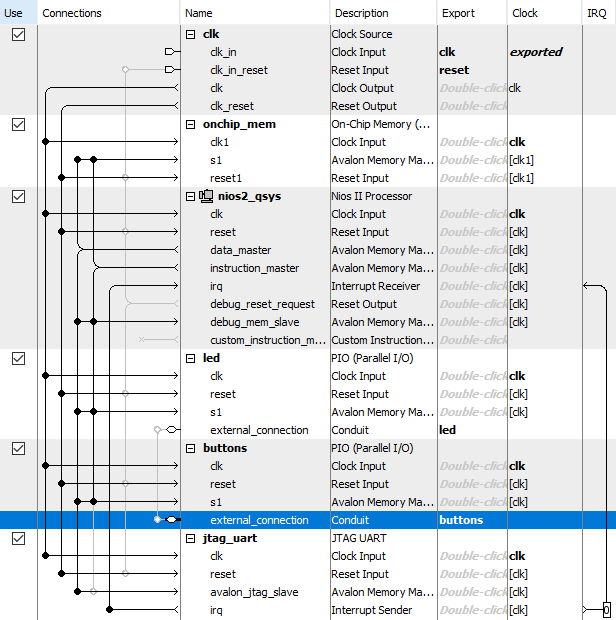
\includegraphics[width=0.95\linewidth]{1}
	\caption{System Contents}
\end{figure}

Итоговый вид Address Map:
\begin{figure}[H]
	\centering
	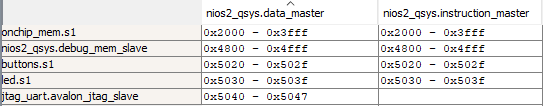
\includegraphics[scale=1]{2}
	\caption{Address Map}
\end{figure}

Сгенерируем Verilog описание созданной системы:
\begin{figure}[H]
	\centering
	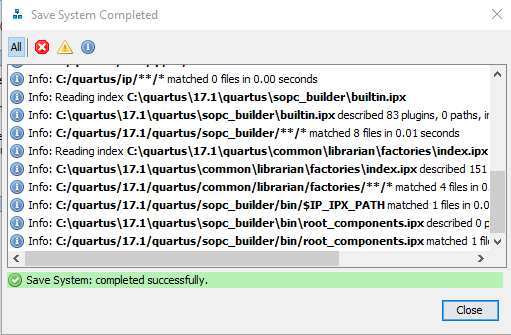
\includegraphics[scale=1]{3}
	\caption{Generate}
\end{figure}

\subsection{Интеграция аппаратной части проекта}

Введем проект, содержащий созданную систему, в графическом редакторе.
\begin{figure}[H]
	\centering
	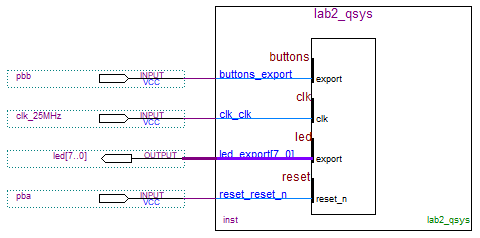
\includegraphics[scale=1]{4}
	\caption{\code{lab2.bdf}}
\end{figure}

Подключим файл с описанием созданной в Qsys системы к проекту и выполним компиляцию проекта.
\begin{figure}[H]
	\centering
	
\includegraphics[scale=1]{5}
	\caption{Результат компиляции}
\end{figure}

Назначим выводы проекта.
\begin{figure}[H]
	\centering
	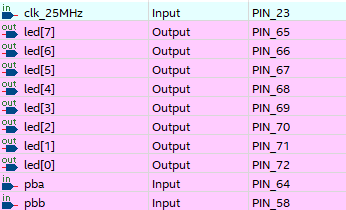
\includegraphics[scale=1]{6}
	\caption{Назначение выводов проекта}
\end{figure}

Интеграция аппаратной части проекта и задание установок проекта завершено.

\subsection{Создание программной части проекта}

Откроем NiosII Software Build Tools for Eclipse и создадим проект с помощью шаблона. Создадим новый файл с исходным кодом. В листинге \ref{code:3} приведен код на языке C.
\newpage
\lstinputlisting[caption=\code{lab3_source.c}, label=code:3]{software/lab3_sw/lab3_source.c}

Обновим настройки проекта и запустим Build.
\begin{figure}[H]
	\centering
	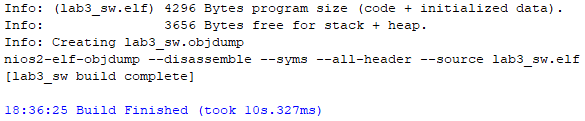
\includegraphics[scale=1]{7}
	\caption{Build}
\end{figure}

\subsection{Конфигурирование СБИС}

Подключим плату к компьютеру и выполним загрузку программы на плату. При каждом нажатии кнопки \code{pbb} происходит изменение номера включенного светодиода от \code{led[0]} к \code{led[7]} на одну позицию с циклическим переходом. Формируется сообщение <<\code{pbb button is pushed}>> в консоли.

\subsection{Анализ и оптимизация размера исполняемого кода программы}

Для проекта \code{lab3_sw_bsp} установим опции BSP по умолчанию.
\begin{figure}[H]
	\centering
	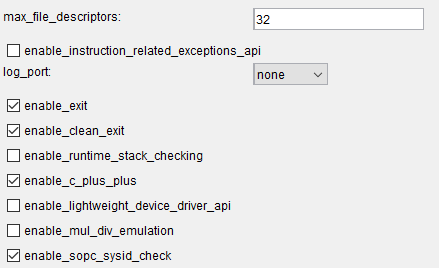
\includegraphics[scale=1]{8}
	\caption{Опции BSP по умолчанию}
\end{figure}

Результаты компиляции показывают, что для исходного кода программы не хватает 39000 байт (конкретное число может быть другим), т.к. размер используемой в проекте памяти для данных, программ, стека установлен 8192 байта

\begin{lstlisting}[caption=Ошибка при компиляции, style=console]
make all 
ld.exe: lab3_sw.elf section `.text' will not fit in region `onchip_mem'
ld.exe: address 0x13704 of lab3_sw.elf section `.rwdata' is not within region `onchip_mem'
ld.exe: address 0x1534c of lab3_sw.elf section `.bss' is not within region `onchip_mem'
ld.exe: address 0x13704 of lab3_sw.elf section `.rwdata' is not within region `onchip_mem'
ld.exe: address 0x1534c of lab3_sw.elf section `.bss' is not within region `onchip_mem'
ld.exe: region `onchip_mem' overflowed by 70476 bytes
collect2.exe: error: ld returned 1 exit status
make: *** [lab3_sw.elf] Error 1
\end{lstlisting}

Вернем настройки обратно, включим опцию Create objdump file и скомпилируем снова. 
\begin{lstlisting}[caption=Результаты компиляции, style=console]
Info: (lab3_sw.elf) 4300 Bytes program size (code + initialized data).
Info:               3652 Bytes free for stack + heap.
Info: Creating lab3_sw.objdump
nios2-elf-objdump --disassemble --syms --all-header --source lab3_sw.elf >lab3_sw.objdump
[lab3_sw build complete]

20:50:39 Build Finished (took 14s.639ms)
\end{lstlisting}

Заменим в исходном файле вызовы \code{printf()} на \code{alt_printf()} и сохраним под именем \code{lab3_sw_alt.c}.
\lstinputlisting[caption=\code{lab3_source_alt.c}]{software/lab3_sw/lab3_source_alt.c}

Выполним компиляцию. Результаты компиляции показывают, что требования к объему памяти для исходного кода программ и инициализационных данных сократилось до 2596 байт. При этом под стек и данные осталось 5592 байт.
\begin{lstlisting}[caption=Результаты компиляции, style=console]
Info: (lab3_sw.elf) 2596 Bytes program size (code + initialized data).
Info:               5592 Bytes free for stack + heap.
Info: Creating lab3_sw.objdump
nios2-elf-objdump --disassemble --syms --all-header --source lab3_sw.elf >lab3_sw.objdump
[lab3_sw build complete]

20:58:44 Build Finished (took 2s.373ms)
\end{lstlisting}

Выберем в настройках Optimization level = 3 и запустим компиляцию снова. Результаты компиляции показывают, что требования к объему памяти для исходного кода программ и инициализационных данных сократилось до 2556 байт. При этом под стек и данные осталось 5632 байт.
\begin{lstlisting}[caption=Результаты компиляции, style=console]
Info: (lab3_sw.elf) 2556 Bytes program size (code + initialized data).
Info:               5632 Bytes free for stack + heap.
Info: Creating lab3_sw.objdump
nios2-elf-objdump --disassemble --syms --all-header --source lab3_sw.elf >lab3_sw.objdump
[lab3_sw build complete]

21:02:34 Build Finished (took 2s.522ms)
\end{lstlisting}

\section{Выводы}

В ходе данной работы были изучены основы построения проекта на базе процессора NIOSII. Сначала был создан проект в QII и настроена аппаратная часть с помощью SOPC Builder, затем аппаратная часть была интегрирована в проект как объект symbol в файл .bdf. Программная часть проекта была создана с помощью NIOSII IDE на языке C. После подключения программной части была выполнена полная компиляция проекта и его проверка на плате. 

\end{document}